\subsection{Box Cut and support relocation }

In the CLAS12 design upgrade the space between the Drift Chambers and the Forward Time-Of-Flight was reduced.
In order to accommodate the LTCC in the new space the original aluminum frame has been modified with a cut, see \F{boxCut}.

Four mirror set, segment 15, 16, 17 and 18 had the mounting structure on the part that was removed.
To re-position these segments new threaded holes has been drilled in the frame, and the old holes have been plugged.

\begin{figure}
	\centering
	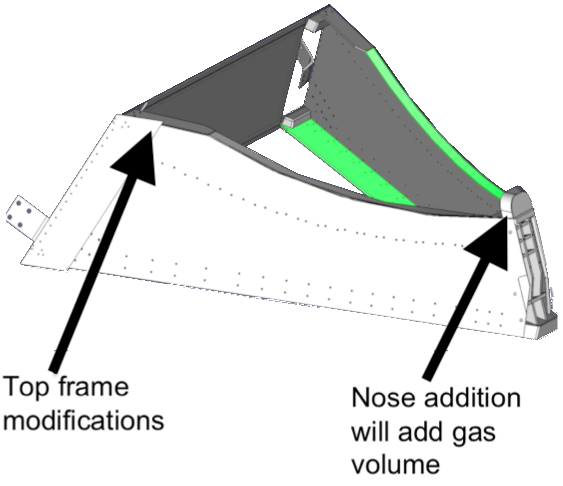
\includegraphics[width=1.0\columnwidth,keepaspectratio]{img/boxCut.png}
	\caption{The LTCC frame modifications. The side-walls had to be cut near the top part of the box from their original
            spherical to a flat outline. The last 3 mirror set had to be relocated. At the bottom of the box, a stainless steel
            nose window support was added to increase the gas volume}
	\label{fig:boxCut}
\end{figure}


\subsection{Nose Addition}

In the original design the upstream window followed the spherical curvature of the frame sidewalls. In the new design, the window is left to inflate
to enlarge the gas volume in order to increase the number of Cherenkov photons. In addition, a ``nose'' support (see \F{boxCut})
has been engineer to increase the gas volume.
The nose dimensions have been optimized to provide the best support while at the same time maximize the gas volume increase. The gas volume increase
of the final configuration is shown in \F{noseVolume}.

\begin{figure}
	\centering
	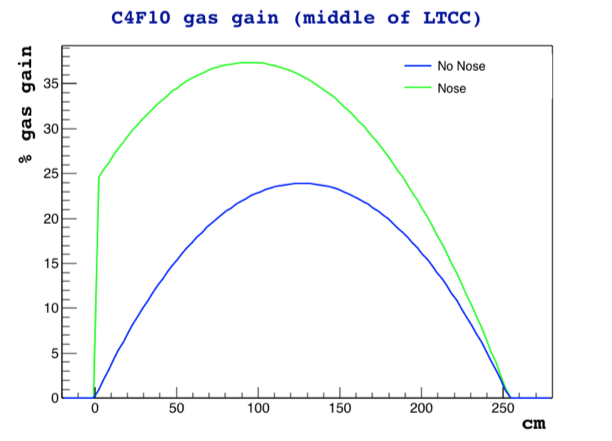
\includegraphics[width=0.95\columnwidth,keepaspectratio]{img/noseVolume.png}
	\caption{The gas volume percentage gains with and without the nose addition compared to the CLAS6 configuration. Blue: the increase due
	          to the window inflation compared to the original flat design. Green: the additional increase due to the nose addition. }
	\label{fig:noseVolume}
\end{figure}


\subsection{Back-wall and Connectors}

Both the high voltage and the signals connectors that link the PMTs inside the hermetical box and the electronics were not
hermetical during CLAS6 operations and epoxy was used to minimize the leaks from these connectors.
As part of the back-wall refurbishment, the patch panel had been rebuilt to accommodate hermetical connectors.

The new back wall design is shown in \F{backWall}. The wall is supported by stainless steel bars that enclose a panel made of foam enclosed by
thin aluminum sheets to minimize the radiation length.
The new patch panels provides 3 connectors for each PMTs: one for High Voltage and two for an identical signal coming from the modified PMT base.
One signal is digitized through Flash ADC and the other one through TDC. The new connectors are hermetical to mitigate the gas leaks in the patch panel.

\begin{figure}
	\centering
	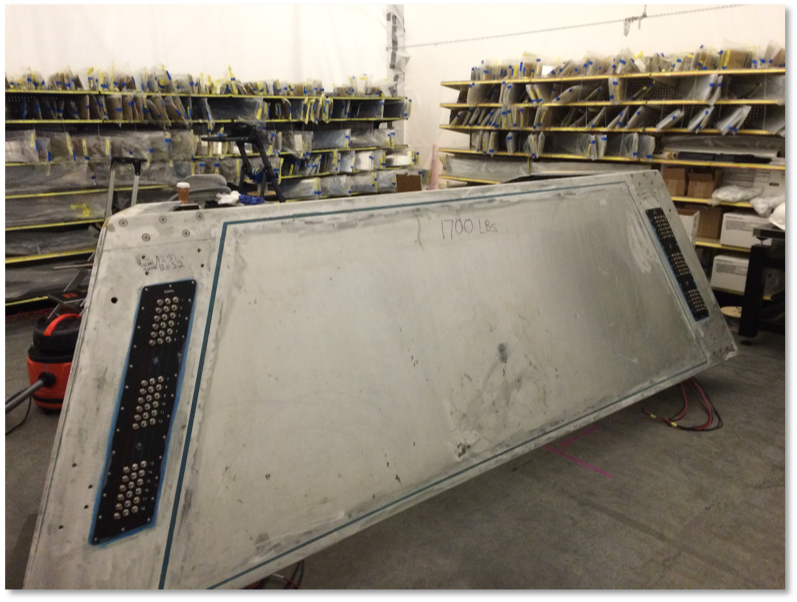
\includegraphics[width=0.95\columnwidth,keepaspectratio]{img/backWall.png}
	\caption{Top view of the back-wall of the LTCC. A stainless steel bar encapsulate a sandwich wall of aluminum and foam. On the left and right side
            of the frame a new patch panel allow for 3 hermetical connectors (1 HV, 2 signals) from each PTM. }
	\label{fig:backWall}
\end{figure}


\subsection{Mirror Support Spine}

When opened for refurbishment, all six LTCC sectors had the mirror support spine broken. The spine was an aluminum honeycomb designed to preventing
the mirror to break under their own weight. It was attached to the box nose and the backwall. The spine was rigid and broke due to small (of the order of 0.5 cm) deformation of the box every time it
is moved.

A new carbon fiber spine has been designed capable to float up to 1 cm due to the box non rigid movement. The mirrors are linked to the spine through stainless steel cables.


\begin{figure}
	\centering
	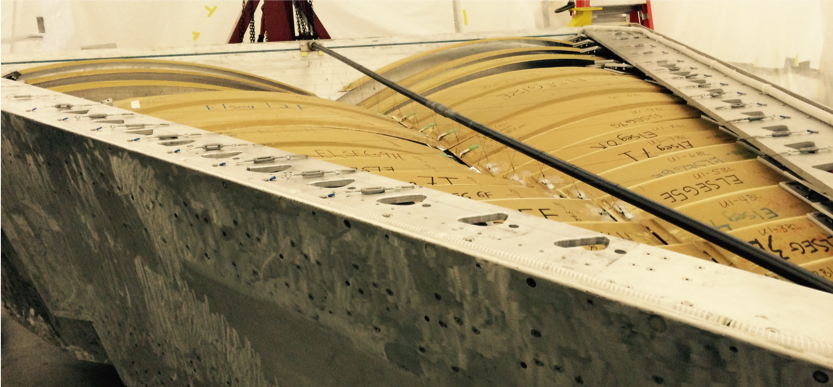
\includegraphics[width=1.0\columnwidth,keepaspectratio]{img/spine.png}
	\caption{Top view of the back-wall of the LTCC. A stainless steel bar encapsulate a sandwich wall of aluminum and foam. On the left and right side
            of the frame a new patch panel allow for 3 hermetical connectors (1 HV, 2 signals) from each PTM. }
	\label{fig:spine}
\end{figure}

The spine was tested by mounting a laser on the box. Its laser line was focused through the elliptical, hyperbolic mirrors to a target in the middle of the covered face of a PMT.
The box was lifted and rotated back and forth by $90$ degrees, see \F{spineTest}. The focused spot on the PMT did not change with any of these movement.

\begin{figure}
	\centering
	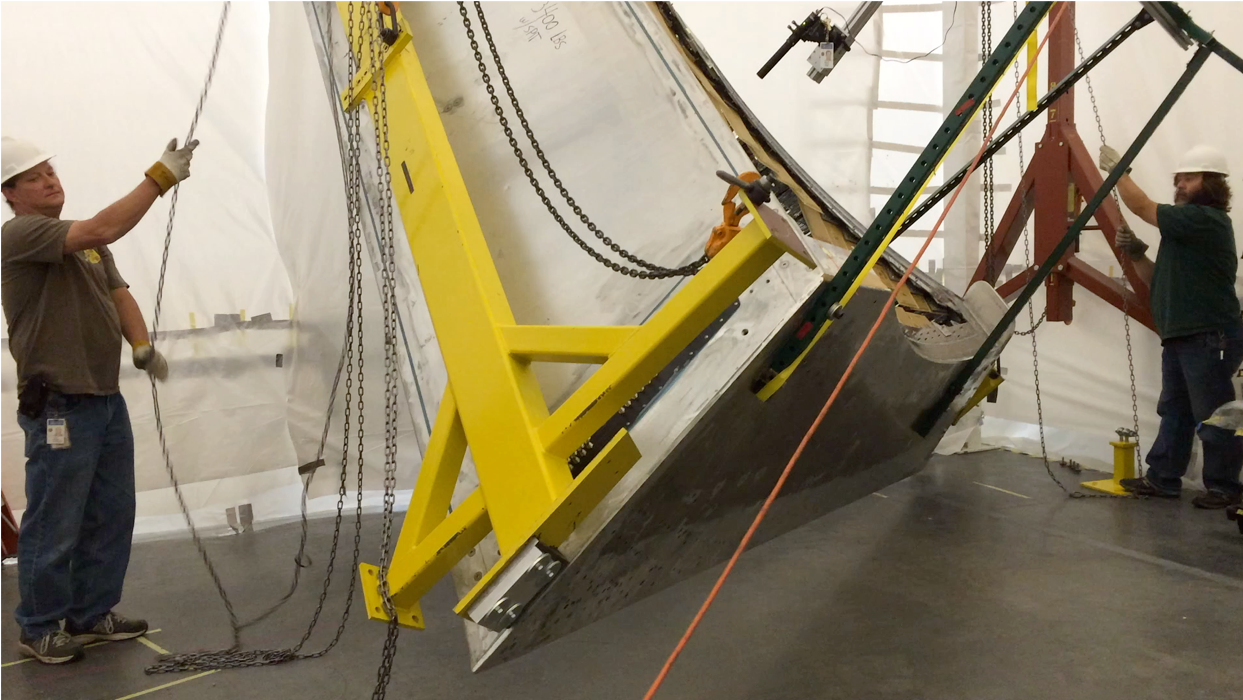
\includegraphics[width=1.0\columnwidth,keepaspectratio]{img/spineTest.png}
	\caption{Spine tests: a laser was mounted on a structure attached to one LTCC sector, pointing a laser line that was focused by the mirrors to a target on the face of one PMTs. The focused laser
            spot never changed during the box movements and rotations.}
	\label{fig:spineTest}
\end{figure}





